\tikzstyle{input_neuron}=[circle,draw=red!50,fill=red!10,thick,minimum size=.2mm]
\tikzstyle{hidden_neuron}=[circle,draw=blue!50,fill=cyan!10,thick,minimum size=1mm]
\tikzstyle{output_neuron}=[circle,draw=green!50,fill=green!10,thick,minimum size=1mm]
\tikzstyle{input}=[circle,draw=black!50,fill=black!20,thick,minimum size=1.5mm]

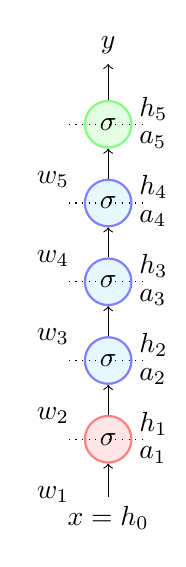
\begin{tikzpicture}

	\node [input_neuron] (neuron0) at (7,5)  {$\sigma$} ;
	\node (input0) at (7,4)  {$x=h_0$};
	
	\node [hidden_neuron] (neuron1) at (7,6)  {$\sigma$};
	\node [hidden_neuron] (neuron2) at (7,7)  {$\sigma$};
	\node [hidden_neuron] (neuron3) at (7,8)  {$\sigma$};
	\node [output_neuron] (neuron4) at (7,9)  {$\sigma$} ;
	
	\node (output0)  at (7,10) {$y$};
	
	\draw [->] (input0) -- (neuron0);
	\draw [->] (neuron0) -- (neuron1);
	\draw [->] (neuron1) -- (neuron2);
	\draw [->] (neuron2) -- (neuron3);
	\draw [->] (neuron3) -- (neuron4);
	\draw [->] (neuron4) -- (output0);
	\draw [dotted] (6.5,5) -- (7.5,5);
	\draw [dotted] (6.5,6) -- (7.5,6);
	\draw [dotted] (6.5,7) -- (7.5,7);
	\draw [dotted] (6.5,8) -- (7.5,8);
	\draw [dotted] (6.5,9) -- (7.5,9);
	\node[text width=0.01cm] at (6.1,4.3) {$w_1$};
	\node[text width=0.01cm] at (6.1,5.3) {$w_2$};
	\node[text width=0.01cm] at (6.1,6.3) {$w_3$};
	\node[text width=0.01cm] at (6.1,7.3) {$w_4$};
	\node[text width=0.01cm] at (6.1,8.3) {$w_5$};
	
	
	\node[text width=0.01cm] at (7.4,4.8) {$a_1$};
	\node[text width=0.01cm] at (7.4,5.2) {$h_1$};
	\node[text width=0.01cm] at (7.4,5.8) {$a_2$};
	\node[text width=0.01cm] at (7.4,6.2) {$h_2$};
	\node[text width=0.01cm] at (7.4,6.8) {$a_3$};
	\node[text width=0.01cm] at (7.4,7.2) {$h_3$};
	\node[text width=0.01cm] at (7.4,7.8) {$a_4$};
	\node[text width=0.01cm] at (7.4,8.2) {$h_4$};
	\node[text width=0.01cm] at (7.4,8.8) {$a_5$};
	\node[text width=0.01cm] at (7.4,9.2) {$h_5$};
	
\end{tikzpicture}